% GenAU training overview (Fig. 2, \label{fig:Model-Arch}).
% Drawn at exactly the CVPR \textwidth (6.875in = 17.4625cm), so that
% 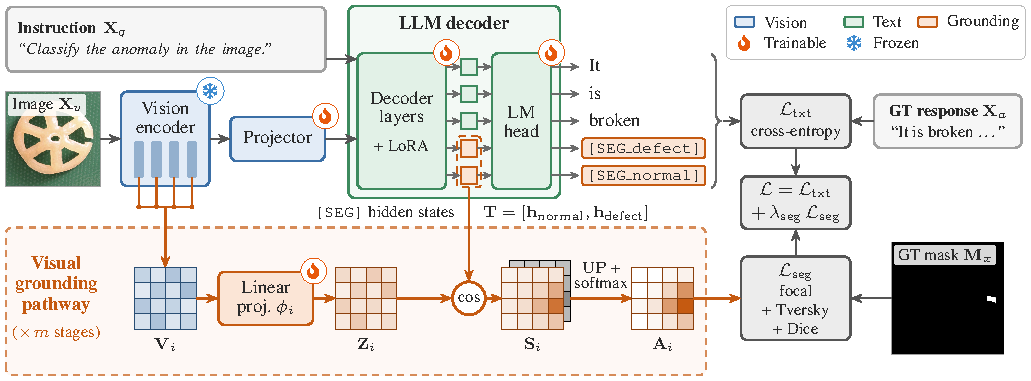
\includegraphics[width=\textwidth]{imgs/GenAU_Arch.pdf} places it at 1:1 and its
% Times text matches the body: 9pt module labels (= caption size), 8pt annotations.
% Build (from this directory):  pdflatex GenAU_Arch.tex   ->  GenAU_Arch.pdf
%
% Layout grid (cm): content inside a 0.1 margin; two rows (text pathway, token
% rows centred at y=4.4; grounding pathway at y=1.4) and, on the right, a loss
% column (x=13.475) and a ground-truth column (x=16.055).
\documentclass[10pt]{standalone}
\usepackage{times}
\usepackage{amsmath,amssymb}
\usepackage{graphicx}
\usepackage{fontawesome5}
\usepackage{tikz}
\usetikzlibrary{arrows.meta,calc,fit,backgrounds,decorations.pathreplacing}

% One hue per pathway (Sec. 3.1): blue = shared vision, green = text pathway,
% orange = visual grounding pathway (the GenAU orange of Fig. 1); grey = data/losses.
\definecolor{ink}{HTML}{2B2B2B}
\definecolor{visS}{HTML}{3B6FA6}\definecolor{visF}{HTML}{E3ECF7}
\definecolor{txtS}{HTML}{3D8A5E}\definecolor{txtF}{HTML}{E2F1E7}
\definecolor{segS}{HTML}{C55A11}\definecolor{segF}{HTML}{FBE5D6}
\definecolor{datS}{HTML}{A0A0A0}\definecolor{datF}{HTML}{F6F6F6}
\definecolor{losS}{HTML}{555555}\definecolor{losF}{HTML}{ECECEC}
\definecolor{fire}{HTML}{E8590C}\definecolor{ice}{HTML}{3D8BD0}

\newcommand{\trainable}{\textcolor{fire}{\faFire}}
\newcommand{\frozen}{\textcolor{ice}{\faSnowflake}}

% 4x4 cell grid: #1 lower-left corner, #2 colour, #3 16 intensities 0-100 (top row first)
\newcommand{\cellgrid}[3]{%
  \begin{scope}[shift={#1}]
    \foreach \v [count=\k from 0] in {#3}{%
      \pgfmathtruncatemacro{\r}{\k/4}%
      \pgfmathtruncatemacro{\c}{mod(\k,4)}%
      \fill[#2!\v!white] (\c*\cs,{(3-\r)*\cs}) rectangle ++(\cs,\cs);
    }
    \draw[#2!70!black, line width=0.3pt] (0,0) grid[step=\cs] (4*\cs,4*\cs);
  \end{scope}}

\begin{document}
\begin{tikzpicture}[
  x=1cm, y=1cm, font=\small, text=ink,
  >={Stealth[length=1.8mm,width=1.4mm]},
  box/.style={draw=#1S, fill=#1F, line width=0.7pt, rounded corners=3pt,
              align=center, inner sep=3pt},
  badge/.style={circle, fill=white, draw=#1, line width=0.45pt, inner sep=0.9pt,
                font=\footnotesize},
  tag/.style={anchor=north west, fill=white, fill opacity=0.85, text opacity=1,
              rounded corners=1pt, inner sep=1.5pt, font=\footnotesize},
  chip/.style={anchor=west, font=\footnotesize\ttfamily, fill=segF, draw=segS,
               line width=0.5pt, rounded corners=1.5pt, inner sep=1.8pt},
  lbl/.style={font=\footnotesize},
  flow/.style={->, draw=ink!80, line width=0.65pt},
  gflow/.style={->, draw=segS, line width=0.85pt},
  short/.style={->, >={Stealth[length=1.3mm,width=1.1mm]}, draw=ink!70, line width=0.5pt},
]
\def\cs{0.26}
\path[use as bounding box] (0,0) rectangle (17.4625,6.45);

% ============================ inputs + shared encoder ============================
\node[box=dat, anchor=north west, text width=5.05cm, align=left, minimum height=1.1cm,
      inner xsep=5pt] (ins) at (0.1,6.35)
  {{\footnotesize\bfseries Instruction $\mathbf{X}_q$}\\[-1pt]
   {\footnotesize\itshape ``Classify the anomaly in the image.''}};

\node[inner sep=0, draw=datS, line width=0.4pt] (img) at (0.9,4.1)
  {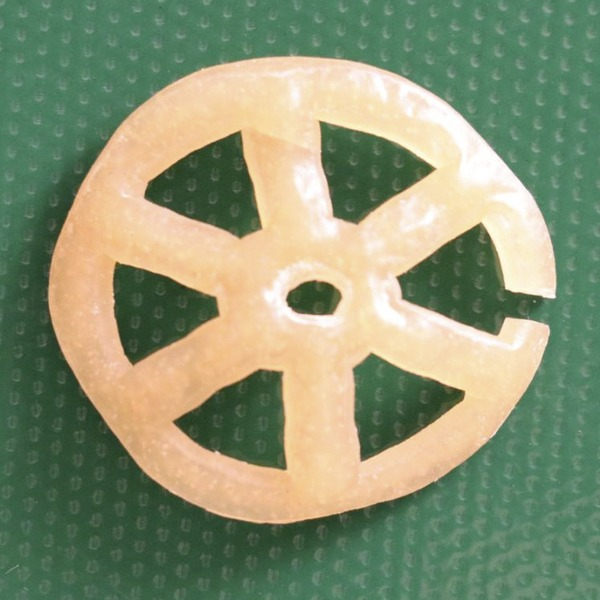
\includegraphics[width=1.6cm]{arch_input.jpg}};
\node[tag] at ($(img.north west)+(0.05,-0.05)$) {Image $\mathbf{X}_v$};

\node[box=vis, minimum width=1.5cm, minimum height=1.6cm] (enc) at (2.8,4.1) {};
\node[anchor=north, align=center] at ($(enc.north)+(0,-0.05)$) {Vision\\[-2pt]encoder};
\foreach \x in {2.35,2.65,2.95,3.25}
  \fill[visS!55, rounded corners=0.8pt] (\x-0.08,3.45) rectangle (\x+0.08,4.05);
\node[badge=ice] at (enc.north east) {\frozen};

\node[box=vis, minimum width=1.6cm, minimum height=0.75cm] (proj) at (4.7,4.1) {Projector};
\node[badge=fire] at (proj.north east) {\trainable};

\draw[flow] (img.east) -- (enc.west);
\draw[flow] (enc.east) -- (proj.west);

% ============================ text pathway (top row) ============================
\begin{scope}[on background layer]
  \fill[txtF!40, draw=txtS, line width=0.7pt, rounded corners=3pt] (5.9,3.1) rectangle (9.48,6.35);
\end{scope}
\node at (7.69,6.06) {\textbf{LLM decoder}};
\node[box=txt, minimum width=1.5cm, minimum height=2.3cm] (dec) at (6.8,4.4)
  {Decoder\\[-2pt]layers\\[3pt]{\footnotesize + LoRA}};
\node[badge=fire] at (dec.north east) {\trainable};
\node[box=txt, minimum width=1.0cm, minimum height=2.3cm] (head) at (8.83,4.4) {LM\\[-2pt]head};
\node[badge=fire] at (head.north east) {\trainable};

\draw[flow] (ins.east |- 0,5.45) -- (dec.west |- 0,5.45);
\draw[flow] (proj.east) -- (dec.west |- proj.east);

% hidden states -> LM head -> response tokens
\foreach \y/\t [count=\i] in {5.32/It, 4.86/is, 4.4/broken, 3.94/, 3.48/}{
  \ifnum\i>3 \def\hc{seg}\else\def\hc{txt}\fi
  \node[draw=\hc S, fill=\hc F, line width=0.5pt, minimum size=0.28cm, inner sep=0] (h\i) at (7.94,\y) {};
  \draw[short] (dec.east |- h\i) -- (h\i.west);
  \draw[short] (h\i.east) -- (head.west |- h\i);
  \draw[short] (head.east |- h\i) -- (9.8,\y);
  \node[anchor=west] at (9.85,\y) {\strut\t};
}
\node[chip] at (9.85,3.94) {[SEG\_defect]};
\node[chip] at (9.85,3.48) {[SEG\_normal]};

% ============================ grounding pathway (bottom row) ============================
\begin{scope}[on background layer]
  \draw[segS!70, dashed, line width=0.6pt, rounded corners=3pt, fill=segF!25]
    (0.1,0.1) rectangle (11.95,2.6);
\end{scope}
\node[align=center, text=segS] at (0.95,1.4)
  {\textbf{Visual}\\[-1pt]\textbf{grounding}\\[-1pt]\textbf{pathway}\\[2pt]{\footnotesize ($\times\,m$ stages)}};

% the m encoder stages, tapped into V_i
\foreach \x in {2.35,2.65,2.95,3.25}{
  \draw[segS, line width=0.6pt] (\x,3.45) -- (\x,2.95);
  \fill[segS] (\x,2.95) circle (0.9pt);
}
\draw[segS, line width=0.6pt] (2.35,2.95) -- (3.25,2.95);
\draw[gflow] (2.8,2.95) -- (2.8,1.92);

\cellgrid{(2.28,0.88)}{visS}{30,18,40,22, 15,35,20,45, 38,22,30,16, 20,42,18,28}
\node[lbl, anchor=north] at (2.8,0.86) {$\mathbf{V}_i$};

\node[box=seg, minimum width=1.6cm, minimum height=0.9cm] (phi) at (4.5,1.4)
  {Linear\\[-2pt]proj.\ $\phi_i$};
\node[badge=fire] at (phi.north east) {\trainable};
\draw[gflow] (3.32,1.4) -- (phi.west);

\cellgrid{(5.68,0.88)}{segS}{22,12,30,16, 10,26,14,34, 28,16,22,10, 14,32,12,20}
\node[lbl, anchor=north] at (6.2,0.86) {$\mathbf{Z}_i$};
\draw[gflow] (phi.east) -- (5.68,1.4);

% cosine similarity with the [SEG] anchors
\node[circle, draw=segS, fill=white, line width=0.85pt, minimum size=0.56cm, inner sep=0,
      font=\footnotesize] (cos) at (7.94,1.4) {cos};
\draw[gflow] (6.72,1.4) -- (cos.west);
\node[draw=segS, dashed, line width=0.5pt, rounded corners=1.5pt, fit=(h4)(h5), inner sep=1.5pt] (seghl) {};
\draw[gflow] (seghl.south) -- (cos.north);
\node[lbl, anchor=east] at (7.82,2.85) {\texttt{[SEG]} hidden states};
\node[lbl, anchor=west] at (8.06,2.85)
  {$\mathbf{T}=[\mathbf{h}_{\mathrm{normal}},\mathbf{h}_{\mathrm{defect}}]$};

% similarity logits S_i (normal / defect channels) -> anomaly map A_i
\cellgrid{(8.62,1.0)}{black}{20,22,18,25, 22,18,20,30, 18,20,25,45, 22,20,18,28}
\cellgrid{(8.5,0.88)}{segS}{8,10,12,15, 10,15,25,50, 12,20,45,85, 8,12,20,35}
\node[lbl, anchor=north] at (9.02,0.86) {$\mathbf{S}_i$};
\draw[gflow] (cos.east) -- (8.5,1.4);
\draw[gflow] (9.66,1.4) -- (10.7,1.4)
  node[midway, above=1pt, align=center, lbl] {$\mathrm{UP}$ +\\[-2pt]softmax};
\cellgrid{(10.7,0.88)}{segS}{0,0,5,8, 0,5,25,65, 5,15,60,100, 0,5,15,35}
\node[lbl, anchor=north] at (11.22,0.86) {$\mathbf{A}_i$};

% ============================ losses (x=13.475) and ground truth (x=16.055) ============================
\draw[decorate, decoration={brace, amplitude=4pt}, ink!70, line width=0.6pt]
  (12.05,5.53) -- (12.05,3.27);
\node[box=los, minimum width=1.85cm, minimum height=0.9cm] (ltxt) at (13.475,4.4)
  {$\mathcal{L}_{\mathrm{txt}}$\\[-1pt]{\footnotesize cross-entropy}};
\draw[flow] (12.25,4.4) -- (ltxt.west);
\node[box=dat, minimum width=2.5cm, minimum height=0.9cm] (gtt) at (16.05,4.4)
  {{\footnotesize\bfseries GT response $\mathbf{X}_a$}\\[-1pt]{\footnotesize ``It is broken \ldots''}};
\draw[flow] (gtt.west) -- (ltxt.east);

\node[box=los, minimum width=1.85cm] (lseg) at (13.475,1.4)
  {$\mathcal{L}_{\mathrm{seg}}$\\[-1pt]{\footnotesize focal}\\[-2pt]{\footnotesize + Tversky}\\[-2pt]{\footnotesize + Dice}};
\draw[gflow] (11.74,1.4) -- (lseg.west);
\node[inner sep=0, draw=datS, line width=0.4pt] (gtm) at (16.05,1.4)
  {
\includegraphics[width=1.9cm]{arch_gtmask.png}};
\node[tag] at ($(gtm.north west)+(0.05,-0.05)$) {GT mask $\mathbf{M}_x$};
\draw[flow] (gtm.west) -- (lseg.east);

\node[box=los, line width=0.8pt, minimum width=1.85cm] (ltot) at (13.475,3.02)
  {$\mathcal{L}=\mathcal{L}_{\mathrm{txt}}$\\$+\,\lambda_{\mathrm{seg}}\,\mathcal{L}_{\mathrm{seg}}$};
\draw[flow] (ltxt.south) -- (ltot.north);
\draw[flow] (lseg.north) -- (ltot.south);

% ============================ legend (top-right) ============================
\begin{scope}[font=\footnotesize]
  \draw[datS!70, line width=0.4pt, rounded corners=2pt] (12.3,5.45) rectangle (17.36,6.35);
  \foreach \c/\t/\x in {vis/Vision/12.45, txt/Text/14.3, seg/Grounding/15.55}{
    \fill[\c F, draw=\c S, line width=0.5pt, rounded corners=1pt] (\x,5.99) rectangle ++(0.32,0.18);
    \node[anchor=west] at (\x+0.36,6.08) {\t};
  }
  \node at (12.61,5.73) {\trainable}; \node[anchor=west] at (12.81,5.73) {Trainable};
  \node at (14.46,5.73) {\frozen};    \node[anchor=west] at (14.66,5.73) {Frozen};
\end{scope}
\end{tikzpicture}
\end{document}
